%%%%%%%%%%%%%%%%%%%%%%%%%%%%%%%%%%%%%%%%%%%%%%%%%%%%%%%%%%%%%%%%%%%%%%%%%%%%%%%%
%2345678901234567890123456789012345678901234567890123456789012345678901234567890
%        1         2         3         4         5         6         7         8

%\documentclass[letterpaper, 10 pt, conference]{ieeeconf}  % Comment this line out if you need a4paper

\documentclass[a4paper, 11pt, conference]{ieeeconf}      % Use this line for a4 paper

%\IEEEoverridecommandlockouts                              % This command is only needed if
                                                          % you want to use the \thanks command

%\overrideIEEEmargins                                      % Needed to meet printer requirements.

%In case you encounter the following error:
%Error 1010 The PDF file may be corrupt (unable to open PDF file) OR
%Error 1000 An error occurred while parsing a contents stream. Unable to analyze the PDF file.
%This is a known problem with pdfLaTeX conversion filter. The file cannot be opened with acrobat reader
%Please use one of the alternatives below to circumvent this error by uncommenting one or the other
%\pdfobjcompresslevel=0
%\pdfminorversion=4

% See the \addtolength command later in the file to balance the column lengths
% on the last page of the document

\usepackage[parfill]{parskip} % Activate to begin paragraphs with an empty line rather than an indent

\usepackage{booktabs} % for much better looking tables


% The following packages can be found on http:\\www.ctan.org
%\usepackage{graphics} % for pdf, bitmapped graphics files
%\usepackage{epsfig} % for postscript graphics files
%\usepackage{mathptmx} % assumes new font selection scheme installed
%\usepackage{times} % assumes new font selection scheme installed
\usepackage{amsmath} % assumes amsmath package installed
\usepackage[utf8]{inputenc}
% scientific unit package
\usepackage{siunitx}
% for images
\usepackage{graphicx}
\usepackage{gensymb}
\usepackage{textcomp}
\usepackage{float}
\usepackage{url}
\usepackage{xcolor}
\usepackage{hyperref}
\hypersetup{
  colorlinks   = true, %Colours links instead of ugly boxes
  urlcolor     = blue, %Colour for external hyperlinks
  linkcolor    = black, %Colour of internal links
  citecolor   = red %Colour of citations
}
%\usepackage{amssymb}  % assumes amsmath package installed

\DeclareSIUnit{\sample}{S}

\title{\LARGE \bf
Deep Learning Lab Exercise 4: Reinforcement Learning}

\author{Ingmar Baetge, Alex Rose}

\begin{document}
\sisetup{quotient-mode=fraction,per-mode=symbol, mode=math}

\maketitle
%\thispagestyle{empty}
%\pagestyle{empty}

%%%%%%%%%%%%%%%%%%%%%%%%%%%%%%%%%%%%%%%%%%%%%%%%%%%%%%%%%%%%%%%%%%%%%%%%%%%%%%%%

\section{CartPole}

We begin the classic control task of CartPole. Instead of imitation learning where the agent analyses expert play to learn the relationship between states and ideal actions (as in Exercise 3), here we use Q-Learning, where the agent samples from a palette of actions in each state, and gradually learns to parameterise a function $Q(State, Action) = Value$. In the CartPole instance our state is a 4-dimensional vector; our function is a simple neural network of two fully-connected 20-unit hidden layers with ReLU activation; and we have two possible actions: \textit{Left} and \textit{Right}.

We also implemented the bonus features:

\begin{itemize}
	\item \textbf{Epsilon Annealing}: in which our probability $\epsilon$ of selecting a random (non-optimal) action is reduced from its starting value by a factor of $3.33 \times 10^{-4}$ after each episode. This gradually shifts the agent's priorities from exploration to exploitation, as time goes on.

	\item \textbf{Boltzmann Exploration}, where instead of selecting randomly with probability $\epsilon$ and optimally with probability $1 - \epsilon$, the agent samples an action according to the SoftMax of its action predictions (with optional SoftMax temperature parameter). This allows the agent to shift from exploration to exploitation only when it becomes more certain about its predicted action-values.

	\item \textbf{Double-Q learning}, where actions are selected using the \textit{current} network, but still evaluated using the \textit{target} network. This decorrelates the noise in the two networks, theoretically avoiding overestimation bias in the $Q$ function.

\end{itemize}

Training was over 1,600 episodes with Adam as our optimiser, learning rate $10^{-4}$, batch size 64, buffer capacity of $100,000$, target network update parameter $\tau=0.01$, and $\epsilon=0.1$ initially. We see that Boltzmann Exploration creates a high performance agent much more quickly than Basic or Double Q Learning, presumably because in the early episodes when the agent has little idea of the best move, Boltzmann encourages it to explore \textit{much} more than a fixed epsilon parameter would allow. Epsilon Annealing, on the other hand, starts out promisingly, but has a disastrous spell later and forgets everything useful it has learned (Figure \ref{fig:train0}). We then tested each agent over 100 episodes, and found that the Boltzmann agent has learned to play perfectly with an average score over 1000, and the Double Q agent, though less impressive, has still solved the problem, with an average score over 200 (Figure \ref{fig:test0}). We should note that these results are very high-variance; in previous runs, we saw agents with identical configurations having very different training curves. Therefore, they should not be taken (for example) as definitive proof that Boltzmann exploration is the best method to solve this problem.

\begin{figure}
  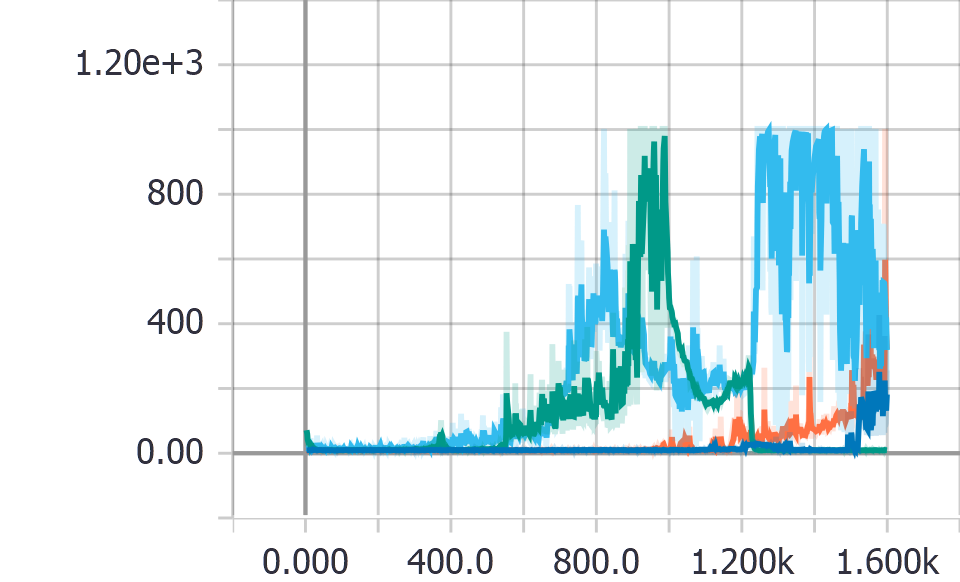
\includegraphics[width=\linewidth]{figs/cartpole_reward.png}
  \caption{Reward over training epochs for Cartpole models: \textcolor{blue}{Default}; \textcolor{teal}{Epsilon Annealing}; \textcolor{cyan}{Boltzmann Exploration}; \textcolor{orange}{Double Q}}
  \label{fig:train0}
\end{figure}

\begin{figure}
  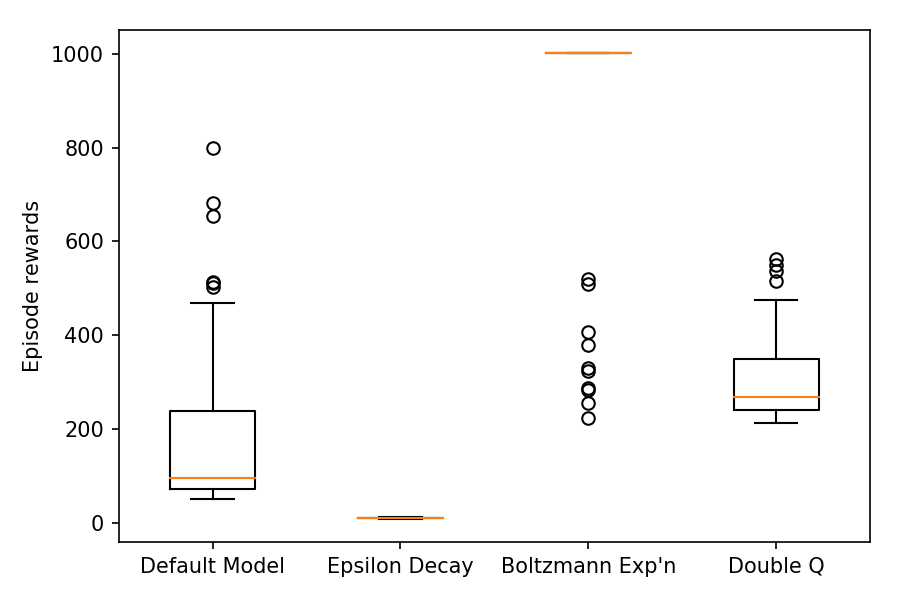
\includegraphics[width=\linewidth]{figs/cartpole_test.png}
  \caption{Test results for Cartpole models}
  \label{fig:test0}
\end{figure}

\section{Car Racing}

We used the same Q learning algorithm, code, and hyperparameters as in CartPole, with modifications to suit the Car Racing environment:

\begin{itemize}
	\item Images preprocessed to greyscale

	\item A deep ConvNet, as described in Table \ref{table:agent1}.

  \item Continuous actions discretised simply to \textit{Nothing, Left, Right, Accelerate, Brake}

  \item A replay buffer of size 500,000.

  \item Frameskip of 2 during training (i.e. every third frame is seen and acted upon, and actions persist over the next two frames). At test time, no frameskip is used.

  \item Training over 1,000 episodes

\end{itemize}

\begin{table}
  \centering
  \caption{Racecar Q-network architecture}
  \label{table:agent1}
  \begin{tabular}{ll}
  Layer & Parameters \\ \hline
  Convolution 1 / ReLU & Filters: 16, Size: 7 \\
  Max Pooling & Size: 2, Stride: 2\\
  Convolution 2 / ReLU & Filters: 32, Size: 5 \\
  Max Pooling & Size: 2, Stride: 2\\
  Convolution 3 / ReLU & Filters: 48, Size: 3 \\
  Max Pooling & Size: 2, Stride: 2\\
  FC layer 1 / ReLU & 512 units\\
  FC layer 2 / ReLU & 128 units\\
  Output & 5 units\\
  \end{tabular}
  \end{table}

For agent testing, we used two methods:

\begin{enumerate}
	\item Actions selected using the maximum prediction from the Q network, leading to discrete actions.
	\item Actions combined using proportions in the Softmax of the last layer, leading to continuous (and noticeably more "noisy") actions.
\end{enumerate}

All seeds (Numpy, TensorFlow and Gym environment) were set to 0 to allow reproducable tests.

\begin{figure}
  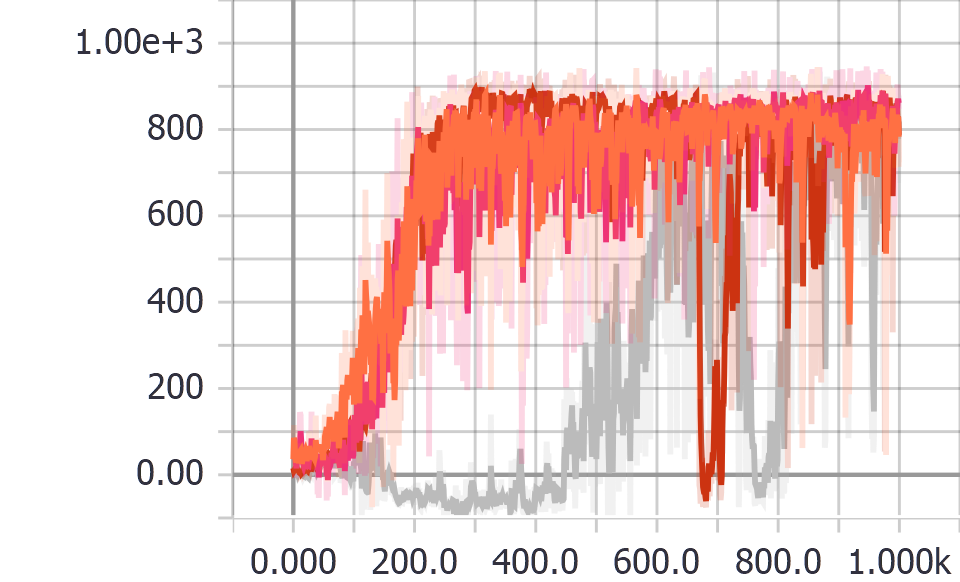
\includegraphics[width=\linewidth]{figs/racecar_train_1234.png}
  \caption{Racecar training curves for \textcolor{orange}{Basic Model}, \textcolor{magenta}{Epsilon Annealing}, \textcolor{red}{Boltzmann Exploration}, \textcolor{gray}{Double Q learning}}
  \label{fig:train1234}
\end{figure}

\begin{figure}
  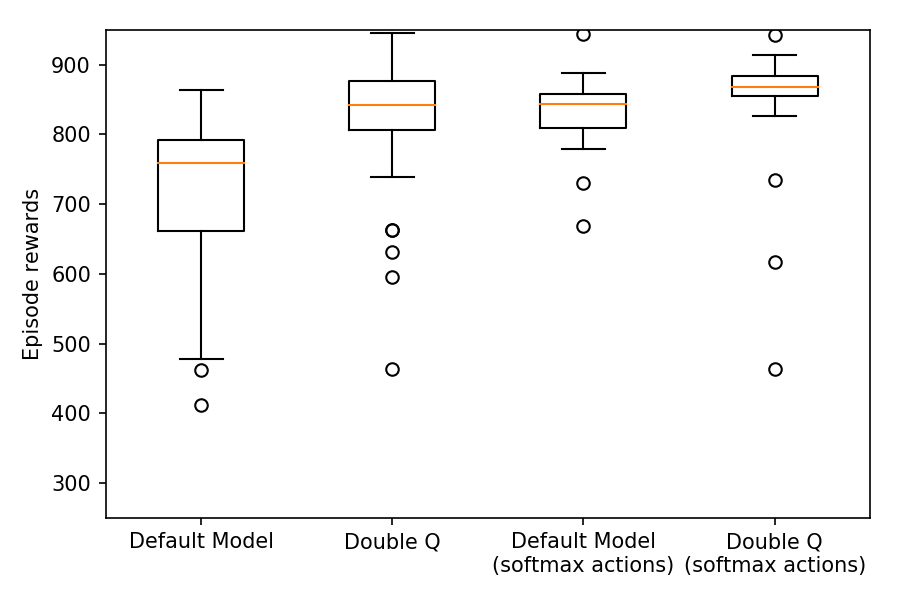
\includegraphics[width=\linewidth]{figs/racecar_1.png}
  \caption{Racecar test results for Basic Model and Double Q learning}
  \label{fig:test1}
\end{figure}

\begin{figure}
  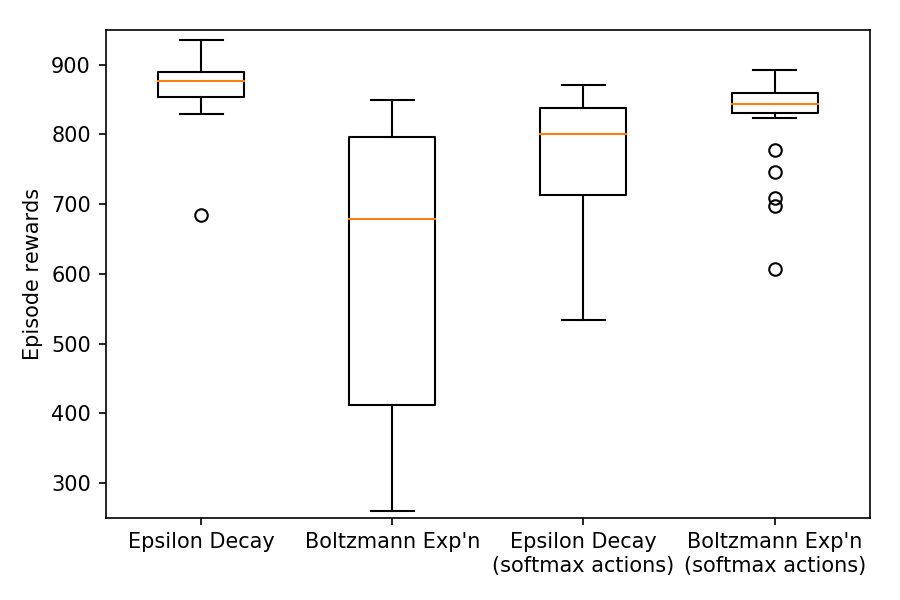
\includegraphics[width=\linewidth]{figs/racecar_2.png}
  \caption{Racecar test results for Epsilon Annealing and Boltzmann Exploration}
  \label{fig:test2}
\end{figure}

Figure \ref{fig:test2} shows our agents doing reasonably well already, with many average scores over 800 (though some agents again "forget" what they've learned during training, and must re-learn it). Notably, Boltzmann exploration does much worse here than in CartPole. One reason is that in Cartpole, for every state there is an unambiguous best action, and once this is found, Boltzmann exploration will quickly allow the agent to exploit it consistently. Whereas in the racecar environment, the reward delta between the best action and other actions can often be quite small, and the agent will be encouraged to explore sub-optimal actions for much longer.

We also notice that these agents are far better at recovery than in the imitation learning exercise, since here they have ample opportunity to learn how to behave in off-road situations (whereas in the imitation learning dataset, there were typically very few examples of the expert's car leaving the road, which left the agent largely unguided when something went wrong).

Observing our agents' driving in test runs, we saw that their characteristic mistake was to enter turns too fast, cut across the corner (missing some reward tiles), and rejoin the road. They learn to do this manoeuvre quite well, and indeed the Q learning algorithm may be encouraging it: doing so allows the agents to avoid slowing down for the corner, and so they pick up rewards as rapidly as possible over a medium time horizon. But by the end of the episode they leave some tiles uncollected, and the clock runs down, diminishing their final reward.

We also see that the 'Softmax' agents tend to drive much more cautiously, and that there is more "noise" in their actions, e.g. rapid light steering on straight stretches of road, just as we would expect. However, they do seem less likely to enter corners too fast than the 'Hardmax' agents. Overall, Softmax action selection does not seem to be systematically better nor worse.

\section{Adding History}

We hypothesise that the agents may be making this corner-cutting mistake because they simply don't have a clear idea of how fast they're going from the single-frame input we've used so far. Therefore, we next implemented image history in order for the agent to better judge its speed, in two different ways:

\begin{enumerate}
	\item Adding the frame immediately prior to the current one to our state buffer, so that the input to our ConvNet is a $(96, 96, \textbf{2})$ image

	\item Subtracting the prior frame from the current one to produce a difference image, and processing this difference image using a separate, smaller ConvNet (which is merged with the first one in the fully connected layers)
\end{enumerate}

Results are shown in Figures \ref{fig:train5678} and \ref{fig:test3}. The model trained with an additional difference frame as input exhibited better acceleration and braking behaviour, and it also showed a reduced tendency to cut corners. It is therefore reasonable to assume that giving the model access to speed information helps the agent learn this improved behaviour.

\begin{figure}
  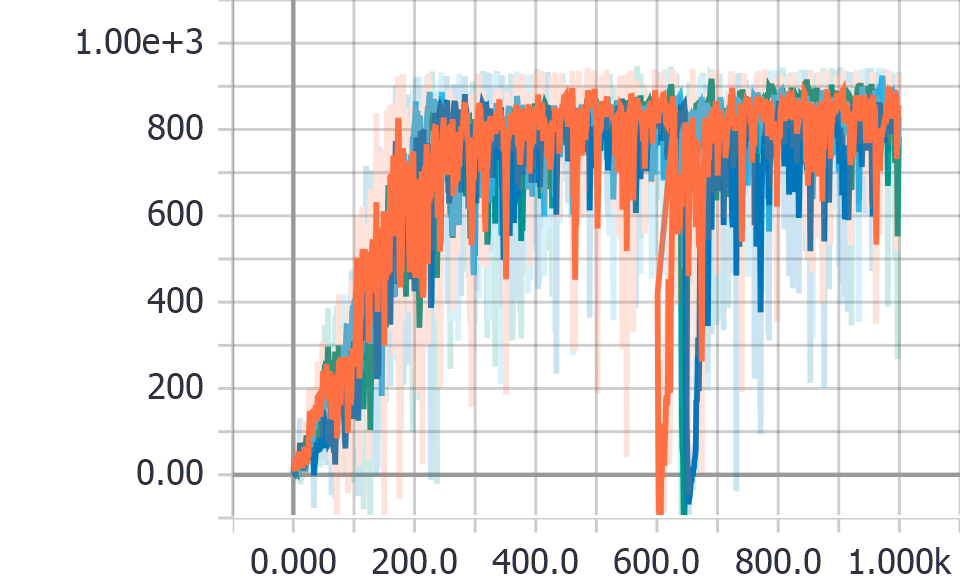
\includegraphics[width=\linewidth]{figs/racecar_train_5678.png}
  \caption{Racecar training curves for \textcolor{blue}{History Frame}, \textcolor{cyan}{Difference Frame}, \textcolor{teal}{Diff. Frame with Penalty}, \textcolor{orange}{DF+P with large network}}
  \label{fig:train5678}
\end{figure}


\begin{figure}
  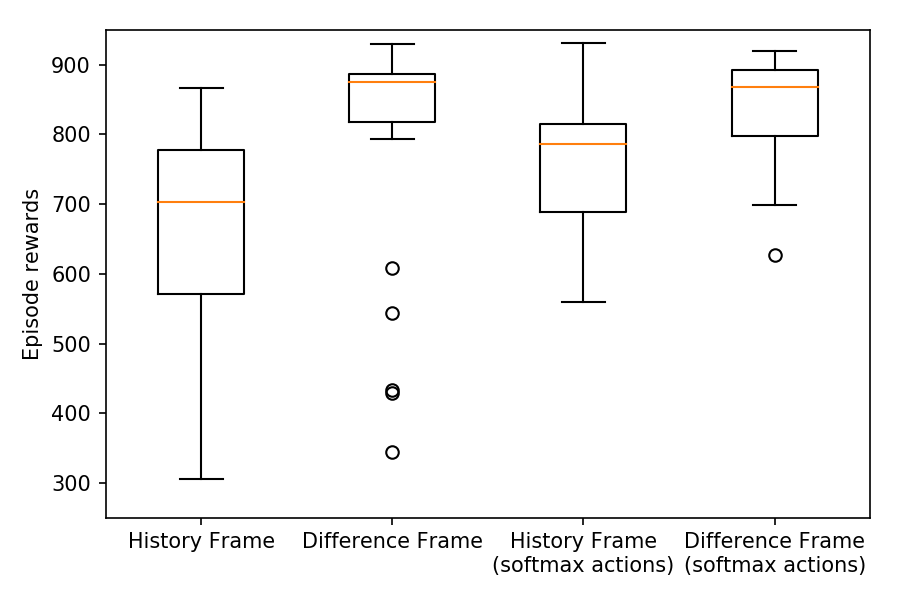
\includegraphics[width=\linewidth]{figs/racecar_3.png}
  \caption{Racecar test results for History Frame and Diff. Frame}
  \label{fig:test3}
\end{figure}

\section{Reward shaping}

We observed that the agent would cut corners quite often - it seemed to learn that there is more benefit in keeping a higher speed, as it will lead to more short term reward, conflicting with the long term goal of collecting every tile of the road, which only becomes relevant towards the end of each episode.

We decided to introduce some reward shaping into the environment - we added two virtual sensors by reading two pixels in front of the car on every step. If these sensors both detect the grass color, a negative reward of $-1$ is added to the total reward, effectively punishing the agent quite strongly for going off road. By adding this simple reward shaping, the agent exhibited less corner cutting, as this behaviour is now penalized. See figure \ref{fig:reward_shaping} for the location of the sensor pixels.

Of course, by implementing reward shaping we have slightly modified the original problem, and encoded some expert guidance or knowledge into the reward function. So in a sense, the Q-learning algorithm is no longer as 'pure'. 

In any case, the question remains: why was reward-shaping necessary? That is, why did Q-learning reward short term gains from corner cutting at the cost of a larger long-term performance hit? The obvious answer is the discount factor of $0.99$ that we used: for example, a missed reward 500 timesteps into the future would be discounted by a factor of $0.99^{500} \approx \frac{1}{152}$. We did also experiment with agents that discounted less or not at all, but these showed worse performance.

A video recording of this Difference Frame + Penalty (DF + P) agent's performance over one episode (the first that we tested) is available in our repository \cite{repo}.

\begin{figure}
  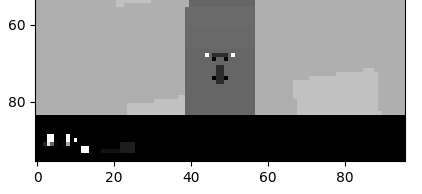
\includegraphics[width=\linewidth]{figs/reward_shaping_closeup.png}
  \caption{Sensor positions for reward shaping: Detecting grass in the two white locations (pixels $(44, 68)$ and $(51,68)$) was penalized with a negative reward of $-1$. As the car position is almost static, the sensor locations were hardcoded.}.
  \label{fig:reward_shaping}
\end{figure}

\begin{figure}
  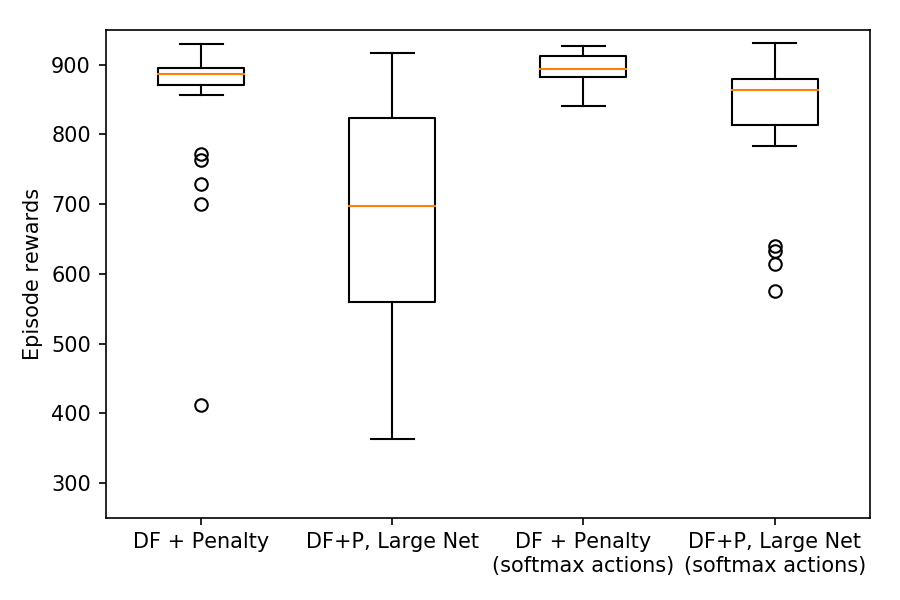
\includegraphics[width=\linewidth]{figs/racecar_4.png}
  \caption{Racecar test results for Diff. Frame + Penalty, DF + P. with large network}
  \label{fig:test4}
\end{figure}

\section{Improving on the Difference Frame + Penalty agent}

In many episodes, the DF + P agent performs a perfect run, driving reasonably fast and picking up every reward tile. Sometimes it still misses a few tiles, especially on sharp corners. We tried improving this with one final model, where we doubled the number of filters in every convolution layer, and increased the number of units in fully connected layers by 50\%. We did this with the hypothesis that the agent may have been unable to learn complex enough representations with the incumbent model to guide its actions, and in the belief that the larger model should be protected from over-fitting by the continuous stream of new training data supplied to the gradient descent algorithm. Unfortunately, as can be seen in Figure \ref{fig:test4}, the larger model was not as successful.

\section*{Conclusion}

Our final results are summarised in Table \ref{table:results}. The best-performing agent was the Difference Frame model with an off-track Penalty (using Softmax action interpretation), and almost as good was the Epsilon-Annealed model (using standard action interpretation), in which no reward shaping was required.

\begin{table}
  \centering
  \caption{Final racecar testing results}
  \label{table:results}
  \begin{tabular}{lrr}
\toprule
         Captions &  Avg Test Score &  Avg Score (Softmax) \\
\midrule
    Default Model &           701.3 &                833.1 \\
    Epsilon Decay &           871.0 &                771.0 \\
  Boltzmann Exp'n &           612.6 &                828.2 \\
         Double Q &           811.5 &                845.6 \\
    History Frame &           650.0 &                754.8 \\
 Difference Frame &           809.5 &                838.3 \\
     DF + Penalty &           855.0 &                895.5 \\
  DF+P, Large Net &           669.2 &                827.3 \\
    DF+P, No Skip &           627.3 &                229.5 \\
\bottomrule
\end{tabular}

  \end{table}

\section*{Acknowledgements}

We would like to thank Guilherme Miotto and Baohe Zhang for all the fruitful discussions, the tutors of this course for their valuable input, and the taxpayers of Germany for the electricity we have consumed.

%%%%%%%%%%%%%%%%%%%%%%%%%%%%%%%%%%%%%%%%%%%%%%%%%%%%%%%%%%%%%%%%%%%%%%%%%%%%%%%%

\begin{thebibliography}{99}

\bibitem{aigym} AI gym car racing: \url{https://gym.openai.com/envs/CarRacing-v0/}

\bibitem{repo} Exercise code: \url{https://github.com/rosea-tf/dl-lab-2018/tree/submit/exercise4_R_NR}

\end{thebibliography}

%%%%%%%%%%%%%%%%%%%%%%%%%%%%%%%%%%%%%%%%%%%%%%%%%%%%%%%%%%%%%%%%%%%%%%%%%%%%%%%%
\end{document}